\section{Problem 1}
\subsection{Problem}
Let $ABC$ be a triangle with incentre $I$. The incircle of the triangle $ABC$ touches the sides $AC$ and $AB$ at points $E$ and $F$, respectively. Let $\ell_B$ and  $\ell_C$ be the tangents to the circumcircle of $BIC$ at $B$ and $C$, respectively. Show that there is a circle tangent to $EF,$ $\ell_B$ and $\ell_C$ with centre on the line $BC$.\nl
\textit{Proposed by Navneel Singhal, India}

\subsection{Common definitions and results}
Let $M$ be the midpoint of $BC$ and $D$ the remaining intouch point (opposite $A$). Let $P$ be the intersection of the angle bisector of $\angle BAC$ and the circumcircle of $ABC$. Let $Q$ be the intersection of the tangents to the circumcircle of $BIC$ in $B$ and $C$. Let $X$, $Y$ and $T$ be the intersections of $EF$ with $\ell_B$, $\ell_C$ and $BC$, respectively.
\nl
It is well known that $P$ is the circumcentre of $BIC$ (by the Incentre-Excentre Lemma\footnote{Let $ABC$ be a triangle, $I$ its incentre and $I_A$ its excentre opposite $A$. The points $B$, $C$, $I$ and $I_A$ lie on a circle centred in the midpoint of the arc $BC$ not containing $A$ on the circumcircle of $ABC$. The proof is by relatively straighforward angle chasing.}). Since $QB$ and $QC$ are tangent to the circumcircle of $BIC$, we have $\angle PBQ=\angle QCP=90^\circ$, which implies $P$, $Q$, $B$ and $C$ are concyclic, therefore $Q$ also lies on the circumcircle of $ABC$. Additionally, by Thales' Theorem, $\angle QAP=90^\circ$ and therefore, $QA\parallel EF$.
\nl
Since $\angle XQY=\angle BAC$ and $\angle YXQ=180^\circ-\angle XQA=\angle ACB$, the triangles $ABC$ and $QYX$ are similar.
\nl
\vfill
\begin{figure}[h]
    \begin{flushright}
        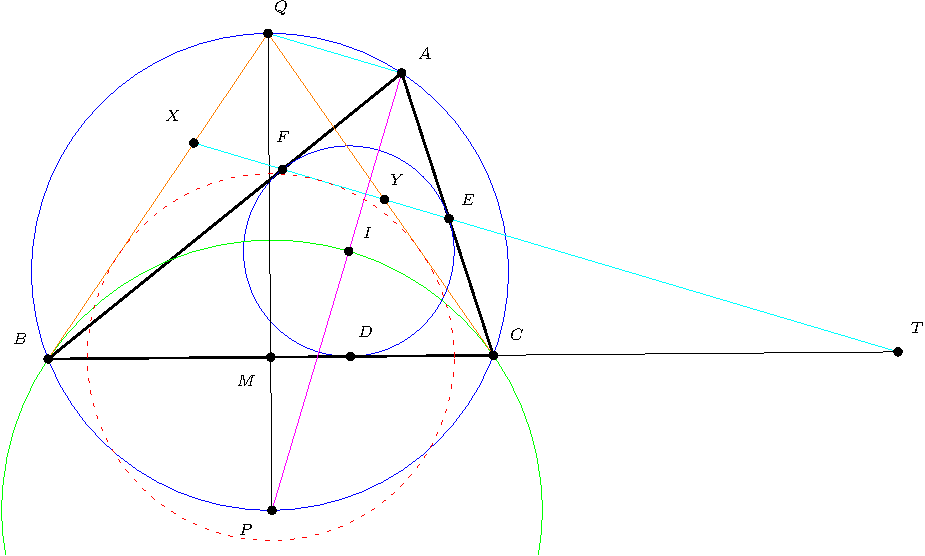
\includegraphics[width=0.9\textwidth]{hard_1_diagram-cropped.pdf}
    \end{flushright}
\end{figure}
\vfill
\newpage
\subsection{Solutions}
\subsubsection{Solution 1 (Fedir Yudin)}
We claim $M$ is the centre of the desired circle. To prove this, we will show the distances of $M$ to $\ell_B$, $\ell_C$ and $EF$ are equal.
\nl
Since $M$ is the midpoint of $BC$, we have
$$d(M, EF)=\frac{d(B, EF)+d(C, EF)}{2}.$$
Let $\alpha=\angle BAI=\angle IAC=\frac{1}{2}\angle BAC$. By considering the lines parallel to $AI$ going through $B$ and $C$, we can see
$$\frac{d(B, EF)+d(C, EF)}{2}=\frac{BF\cdot\cos\alpha+CE\cdot\cos\alpha}{2}=\frac{(BD+DC)\cos\alpha}{2}=MB\cos\alpha,$$
where the last equality holds since $BF=BD$ and $DC=EC$.
\nl
Since $QB$ is tangent to the circumcircle of $BIC$, we have
$$\angle BQM=90^\circ-\angle CBQ=90^\circ-(180^\circ-\angle BIC)=90^\circ-\angle CBI-\angle ICB=\alpha.$$
We conclude by noting that $MBQ$ and the triangle formed by $BM$, $\ell_B$ and the perpendicular from $M$ to $\ell_B$ are similar, which implies
$$MB\cos\alpha=d(M, \ell_B).$$
Due to symmetry, it is clear that $d(M, \ell_B)=d(M, \ell_C)$. Therefore, by combining the above relations, we obtain
$$d(M, EF)=d(M, \ell_B)=d(M, \ell_C).$$
Thus, $M$ is indeed the centre of the desired circle.
\nl
\subsubsection{Solution 2 (Navneel Singhal, Jakob Jurij Snoj)}
Let $\ell$ be the line tangent to the circumcircle of $BIC$ in $I$, which is clearly parallel to $EF$ and $AQ$. Since $\angle PQC=\angle PAC=\angle IAE$ and $\angle AEI=90^\circ=\angle QCP$ due to $PQ$ being the diameter of the circumcircle of $ABC$, the triangles $AEI$ and $QCP$ are similar.
\nl
Since $AEI$ and $QCP$ are similar triangles and $BC$ and $EF$ their altitudes, we can now compute:
$$\frac{d(Q, EF)}{d(Q, \ell)}=\frac{d(A, EF)}{d(A, \ell)}=\frac{QM}{QP}.$$
\nl
Observe the homothety centred in $Q$ taking $P$ to $M$. As it preserves tangency, it sends the circumcircle of $BIC$ to another circle $\omega$, tangent to $\ell_B$ and $\ell_C$, centred in $M$. Additionally, due to the above equality, it sends $\ell$ to $EF$. Since $\ell$ is tangent to the circumcircle of $BIC$, $EF$ is tangent to $\omega$. It follows that $\omega$ is the desired circle.
\subsubsection{Solution 3 (Massimiliano Foschi, Navneel Singhal)}
Note $B$, $C$, $E$ and $X$ are concyclic since $\angle BXE=180^\circ-\angle ACB$.
\nl
Observe that, since $AD$, $BE$ and $CF$ are concurrent, the harmonic property of complete quadrilaterals implies $T$ and $D$ are harmonic conjugates with respect to $A$ and $B$. In particular, we have $TD\cdot TM=TB\cdot TC$, since $TD$ and $TM$ are harmonic and arithmetic means, respectively, of $TB$ and $TC$.
\nl
By taking the power of point $T$ with respect to the circumcircle of $BCEX$, we now obtain
$$TE\cdot TX=TB\cdot TC=TM\cdot TD,$$
which implies $E$, $X$, $M$ and $D$ are concyclic.
\nl
We can now obtain
$$\angle MXE=\angle CDE=\frac{180^\circ-\angle ACB}{2}=\frac{\angle BXE}{2},$$
which implies $XM$ is the angle bisector of $\angle BXY$. Analogously, we obtain $YM$ is the angle bisector of $\angle XYC$. This implies $M$ is the centre of the $Q$-excircle of $QXY$, which concludes the proof.
\subsubsection{Solution 4 (Pitchayut Saengrungkongka)}
Since $AQ$ is parallel to $EF$, we have
$$\frac{FX}{QA}=\frac{BF}{BA}\qquad\text{and}\qquad \frac{EY}{QA}=\frac{CE}{CA}.$$
By Menelaus' Theorem for triangle $AEF$ and line $BC$, we have
$$\frac{AC}{CE}\cdot\frac{ET}{TF}\cdot\frac{FB}{BA}=1,$$
which, along with the above equalities, implies
$$\frac{TE}{TF}=\frac{EY}{FX}.$$
Let $M'$ be the excentre of the $Q$-excircle of $QXY$ (the desired circle). Since
$$\angle M'XY=\frac{\angle BXY}{2}=\frac{\angle BQA}{2}=\angle CDE=\angle DFE,$$
$XM'$ is parallel to $FD$. We conclude by noting the homothety centred in $T$ which takes $E$ to $Y$ evidently also takes $F$ to $X$ and $D$ to $M'$. It follows that $M'$ indeed lies on $BC$ as desired.
\subsubsection{Solution 5 (Pitchayut Saengrungkongka)}
Since $AQ$ is parallel to $EF$, we have
$$\angle XFB=\angle QAB=\angle QCB=\angle TBX,$$
therefore, $BXT$ and $FXB$ are similar triangles. Similarly, we can prove $\angle YEC=\angle TCY$, therefore $TCY$ and $YEC$ are similar triangles. It follows
$$TX=TB\cdot \frac{BX}{FB}\quad\text{and}\quad FX=FB\cdot\frac{XB}{BT},\quad\text{therefore}\quad\frac{TX}{FX}=\frac{TB^2}{BF^2}.$$
Similarly, we obtain $TY/EY=TC^2/CE^2$. We will now prove these two quantities are equal.
\nl
As in Solution 3, we prove $(B, C; D, T)=-1$. It follows that
$$\frac{TX}{FX}=\frac{TB^2}{BF^2}=\frac{TB^2}{BD^2}=\frac{TC^2}{CD^2}=\frac{TC^2}{CE^2}=\frac{TY}{EY}.$$
We conclude analogously to Solution 4 by defining $M'$ and observing the homothety from $T$ taking $X$ to $F$ and $Y$ to $E$ also takes $M'$ to $D$, therefore, $M'$ lies on $BC$ as desired.
\subsubsection{Solution 6 (Pitchayut Saengrungkongka)}
As in the other solutions, we prove $(B, C; D, T)=-1$. It follows that
$$MD\cdot MT=MB\cdot MC=MP\cdot MQ,$$
which implies $MDP$ and $MTQ$ are similar triangles (in particular, this shows $D$ is the orthocentre of $PQT$).
\nl
Let $I_A$ be the centre of the $A$-excircle of $ABC$. It is well known that the incircle and excircle tangency points on a triangle side are symmetric with respect to the side's midpoint. A homothety centred in $A$ sends $D$ to the point diametrically opposite the excircle tangency point on $BC$ on the $A$-excircle of $ABC$, which implies this point is collinear with $A$ and $D$. Together with the above, this implies $MI_A$ and $AD$ are parallel by observing a homothety with ratio $1/2$ centred in the tangency point of the $A$-excircle and $BC$.\nl
The triangles $DIA$ and $MPI_A$ therefore have pairwise parallel sides and are thus similar. In particular, let $G$ be the intersection of $BC$ and $AI$. The point $G$ is the centre of the homothety taking $DIA$ to $MP_IA$, which implies $$\frac{DG}{GM}=\frac{AG}{GI_A}.$$
Recall once again $PMD$ and $TMQ$ are similar triangles, as well as $\angle HTM=\angle APH$. This implies $DG/GM=QH/HM$ and therefore,
$$\frac{QH}{HM}=\frac{AG}{GI_A}.$$
We conclude by noting the triangles $ABC$ and $QYX$ are similar. Indeed, $$\angle ACB=180^\circ-\angle BQA=180^\circ-\angle BXY=\angle YXQ\quad\text{and}\quad  \angle XQY=\angle BAC.$$
Since $AI$ and $QM$ are respective angle bisectors in these triangles, the equality $QH/HM=AG/GI_A$ implies that, since $I_A$ is the excenter opposite $A$ of $ABC$, $M$ is the excenter opposite $Q$ of $QXY$. The $Q$-excircle of $QXY$ is precisely the desired circle, which concludes the proof.

\subsubsection{Solution 7 (Pitchayut Saengrungkongka)}

We use barycentric coordinates with respect to $\triangle ABC$, i.e. point $(x,y,z)$ where $x+y+z=1$ will refer to $x\vec{A}+y\vec{B}+z\vec{C}$. We also use the notation $(kx:ky:kz)$ to denote point $(x,y,z)$ for any $k\in\mathbb{R}$.
\nl
Set $a=BC, b=CA, c=AB$. It's easy to see that $I=(a:b:c)$, $E=(s-c:0:s-a)$ and $F=(s-b:s-a:0)$. Now we proceed to compute $Q$. Since $Q$ lies on the $A$-external bisector, it follows that $Q=(t:-b:c)$ for some $t\in\mathbb{R}$. As in Solution 2, we get that $Q$ lies on the circumcircle of $ABC$. Thus by plugging in this into the circumcircle equation, we get 
$$a^2(-b)(c) + b^2(t)(c) + c^2(-b)(t)=0 \implies t = \frac{a^2}{c-b}$$
Thus $Q$ has coordinate $(-a^2: b(b-c):c(c-b))$. Now to compute $X$, one could intersect $BS$ with $EF$ directly. But this requires factorization of asymmetric expression, so we will present a simpler approach: let $X'$ be the point on $BS$ such that $MX'\parallel DF$ and we aim to show that $X'\in EF$.
\nl
To compute $X'$, note that since $X'\in BS$, there exists $t\in\mathbb{R}$ such that $X' = (-a^2:t:c(c-b))$. Clearly, $M$ has the coordinate $(0:1:1)$ while $\infty_{DF}$ has the coordinate $(a:c-a:-c)$ (as it's also the point at infinity along the $B$-external bisector). By Shoelace formula, we get that
$$0 = \det\begin{bmatrix}
    0 & 1 & 1 \\
    a & c-a & -c \\
    -a^2 & t & c(c-b)
\end{bmatrix}  = a\det\begin{bmatrix}
    0 & 1 & 1 \\
    1 & c-a & -c \\
    -a & t & c(c-b)
\end{bmatrix}
$$ 
Expanding via minors (on the first row), we find that
$$\det\begin{bmatrix}
    1 & -c \\
    -a & c(c-b)
\end{bmatrix} = \det\begin{bmatrix}
    1 & c-a \\
    -a & t
\end{bmatrix} \implies t+a(c-a) = c(c-b)-ac$$
Thus $t=a^2+c^2-bc-2ac$. Therefore $X' = (-a^2 : a^2+c^2-bc-2ac : c(c-b))$. To show that this point lies on $EF$, we need to show that
$$\det\begin{bmatrix}
    -a^2 & a^2+c^2-bc-2ac & c^2-bc \\
    s-c & 0 & s-a \\
    s-b & s-a & 0
\end{bmatrix} = 0$$
Expanding the determinant, we have to show that
$$(a^2+c^2-bc-2ac)(s-a)(s-b)+c(c-b)(s-c)(s-a)=-a^2(s-a)^2.$$
Dividing by $s-a$, and multiplying both sides by $2$, it suffices to show that
$$(a^2+c^2-bc-2ac)(a+c-b) + c(c-b)(a+b-c) + a^2(b+c-a)=0.$$
The first term is
\begin{align*}
    (a^2+c^2-bc-2ac)(a+c-b) &= (a^3+ac^2-abc-2a^2c)+(a^2c+c^3-bc^2-2ac^2) \\
    &\qquad - (a^2b+c^2b-b^2c-2abc) \\
    &= a^3-ac^2+abc-a^2c+c^3-2bc^2-a^2b+b^2c
\end{align*}
while the last two terms combined is
\begin{align*}
    &c(ac+bc-c^2-ab-b^2+bc) + a^2(b+c-a) \\ =\ &  ac^2+2bc^2-c^3-abc-b^2c+a^2b+a^2c-a^3
\end{align*}
It's clear that all add up to $0$ so we get that $X'\in EF$ so $X'=X$. This completes the problem as we have $MX\parallel DF$ thus $\angle MXE = \angle DFE = 90^{\circ}-\tfrac C2$ and $\angle MXY = \angle AQX = \angle C$ hence $MX$ bisects $\angle BXE$.
\subsubsection{Solution 8a (Navneel Singhal)}
We first prove another stronger property of the configuration: the circumcircle of $QXY$ is tangent to the circumcircle of $BIC$.
\nl
Note that, by the Right Angles on Intouch Chord Lemma, we need to show the following:
\nl
Let $ABC$ be a triangle, and let $A'B'C'$ be its orthic triangle, and $H$ its orthocenter. Let the tangents to the circumcircle of $BHC$ at $B$ and $C$ and the line $B'C'$ form a triangle $GUV$, with $G$ being on both tangents, and $V$ being on that from $C$. Then the circumcircle of $GUV$ is tangent to the circumcircle of $BHC$.
\nl
This can be done using Casey's theorem, however we follow a more synthetic approach.\nl
We claim that the point of tangency is $K$, the $A$-Humpty point. 
Let $U'$ be the point where $B'C'$ meets the circumcircle of $BFKM$ (where $M$ is the midpoint of $BC$). Then we have $\angle U'BK = \angle U'C'K = \angle B'C'K = \angle B'AK = \angle KCB = \angle UBK$, so $U = U'$.
\nl
Also $\angle UKB = \angle UKC' + \angle C'KB = \angle UBC' + \angle C'MB = \angle B - \angle A + 2\angle C'CB = \angle C = \angle B'CK + \angle KCB = \angle UVK + \angle KCB$, so the circumcircle of $UKV$ is tangent to the circumcircle of $BKC$, which is also the circumcircle of $BHC$.
\nl
Now by Miquel's theorem on triangle $GBC$ and points $U, V, M$, we have $K$ on the circumcircle of $GUV$ too, so we are done.
\nl
We now conclude by noting that $\angle BUM = \angle BC'M = \angle MBC' = \angle MUE$ (which does not need the full power of the result), or by simply using the properties of the mixtilinear excircle (the midpoint of the touchchord of the mixtilinear excircle is the corresponding excentre).
\subsubsection{Solution 8b (Pitchayut Saengrungkongka)}
Let $E_1$ and $F_1$ be the intersections of $BI$ and $CI$, respectively, with $EF$. Note that, by the Right Angles on Intouch Chord Lemma, we have $MB=MC=ME_1=MF_1$.
\nl
It follows that
$$\angle CME_1=180^\circ-\angle E_1MB=2\angle MBI=\angle MBA=\angle CYE,$$
therefore, the points $C$, $M$, $Y$ and $E_1$ are concyclic. We can now conclude by noting
$$\angle XYM=\angle E_1CM=\angle ME_1C=\angle MYC,$$
from which it follows that $YM$ is the angle bisector of $XYC$. By showing analogously that $XM$ is the angle bisector of $BXY$ or remarking $QM$ is the angle bisector of $BQC$, it follows that $M$ is indeed the desired excentre.
\subsubsection{Solution 8c (Navneel Singhal)}
We define $E_1$ and $F_1$ as in Solution 8b. Since $AQ\parallel EF$, it follows by Reim's Theorem that $B$, $F$, $Y$ and $C$ are concyclic. By the extended Right Angles on Intouch Chord Lemma, $E_1$ lies on the line connecting the midpoints of $BC$ and $CA$. Since this line is parallel to $BF$, it follows by Reim's Theorem that $M$, $C$, $E_1$ and $Y$ are concyclic. We now finish as in Solution 8b.
\subsubsection{Solution 9 (Pitchayut Saengrungkongka)}
Let $H$ be the orthocenter of $BIC$, $K$ be the midpoint of $BH$ and $B_1, C_1$ be the feet of perpendiculars from $C$ to $HB$ and $B$ to $HC$. From the Right Angles on Intouch Chord Lemma, $B_1$,  $C_1$, $E$, $F$ are colinear.
\nl
As $DI\perp BC$, the points $K$, $M$, $D$, $B_1$ and $C_1$ all lie on the nine-point circle of $BCH$. We now apply Pascal's theorem on $KMDB_1C_1K$ to get that $KM \cap EF$, $MD \cap C_1K$ and $KK \cap DB_1$ are collinear. Note that, since $D$, $I$, $B_1$ and $C$ are concyclic,
$$\angle CDB_1 = \angle CIB_1= 180^\circ-\angle BIC=\angle CBI+\angle ICB=90^\circ-\angle BAI90^\circ-\angle BQP=\angle CBQ,$$ so $BQ \parallel DB_1$. Now, since $KD=KB_1$ due to Thales' Theorem, $K$ is the midpoint of arc $DC_1B_1$ in the nine-point circle of $BIC$. It follows the tangent at $K$ to it is parallel to $DB_1$. From the result we obtained by using Pascal's Theorem, it now follows that $KM\cap EF=X$.
\nl
Since
$$\angle C_1B_1I=\angle C_1HI=\angle C_1HD=\angle C_1CD=\angle ICD=\angle IB_1D,$$ $HC$ is one of the angle bisectors of $EF$ and $DB_1$. Since $DB_1\parallel BQ$ and $CH\parallel MK$ and since $X=KM\cap EF$ lies on $BQ$, it follows that $XM$ is also an angle bisector of $\angle BXY$. It follows that $M$ is the desired excentre, which concludes the proof.
\subsubsection{Solution 10 (Amirhosein Rajabi)}
Without loss of generality, we can assume $\angle B \ge \angle C$. One can see that $AQ$ is parallel to $EF$ and we have that since $\angle AEX = \angle QBC$, $XECB$ is a cyclic quadrilateral. Let the bisectors of the angles between $EF$ and $BQ$ intersect $BC$ at $L$ and $N$ (with $L$ between $B$ and $T$). Therefore, $(T, B; L, N) = -1$. Also it is known that $(T, D; B, C) = -1$. Now we use the similarity of triangles $TXB$ and $TCE$ (because of the cyclic quadrilateral $XECB$) along with these harmonic ratios to obtain
\begin{align*}
    \frac{BT}{BD} = \frac{TC}{CD}
    = \frac{TC}{CE}
    = \frac{TX}{XB}
    = \frac{TL}{LB}
    = \frac{NT}{BN}
    = \frac{NB + BT}{DN + BD}
    = \frac{NB}{DN}
\end{align*}
This means $\frac{NT}{BN} = \frac{NB}{DN}$, which gives us $NB^2 = ND \cdot NT$. So the reflection of $B$ over $N$ is the point $C'$ such that $(B, C'; D, T) = -1$, and since $(B, C; D, T) = -1$, we have $C = C'$, so $N$ is the midpoint of $BC$, and we are done.
\subsection{Preliminary notes on grading this problem}
\begin{enumerate}
    \item Any complete solutions should be awarded a full 7 points, regardless of whether they fit in the marking scheme or not.
    \item Partial credits across different approaches are \textbf{not} additive. If a student has a partial solution that can be graded via different marking schemes, the one which leads to the highest score should be followed.
    \item Any partial solutions that can lead to solutions, but which are not outlined in one of the following cases, should be graded equivalently.
    \item If you are not sure if a partial solution can lead to a solution or not, you could discuss this with other graders and if that turns out to be inconclusive, the members of the problem selection committee.
    \item Non-trivial but minor errors in a complete solution usually lead to a deduction of 1 point.
    \item No points are deducted if a contestant fails to handle possible configuration issues (such as not using directed angles).
    \item No points are deducted for quoting well known results without proof (including, but not limited to, Right Angles on Intouch Chord Lemma, Incentre-Excentre Lemma and the harmonic property of complete quadrilaterals).
    \item \textbf{Caveat:} Points for computational approaches should only be awarded if the results are interpreted synthetically.
\end{enumerate}

\subsection{Marking scheme}
In every sub-enumeration, the mentioned partials are given, if the mentioned part of the solution has not been completed. For example, if in the first solution, someone has not expressed $d(M, EF)$ as described, but has proven $d(M, EF)=(d(B, EF)+d(C, EF))/2$, the contestant would get 1 point for that part of the solution. The points within the sub-enumerations are \textbf{not} additive, unless mentioned explicitly.

\subsubsection{Solution 1 (Fedir Yudin)}
\begin{enumerate}
        \marking{1}{Expressing $d(M, l_B)$ or $d(M, l_C)$ only in terms of $MB$, $MC$ or $BC$ and $\alpha$ (such as $MB\cos\alpha$)}
        \marking{5}{Expressing $d(M, EF)$ only in terms of $MB$, $MC$ or $BC$ and $\alpha$ (such as $MB\cos\alpha$)}
        \begin{enumerate}
                \marking{1}{Proving $d(M, EF)=(d(B, EF)+d(C, EF))/2$}
                \marking{3}{Proving $d(M, EF)=((BF+CE)\cos\alpha)/2$}
        \end{enumerate}
        \marking{1}{Argumenting $d(M, \ell_B)=d(M, \ell_C)=d(M, EF)$, which implies $M$ is the desired centre (this point can only be given if 1. and 2. are both proven)}
\end{enumerate}
\subsubsection{Solution 2 (Navneel Singhal, Jakob Jurij Snoj)}
\begin{enumerate}
        \marking{1}{Proving $AQ\parallel EF$ \textbf{and} proving $Q$ lies on the circumcircle of $ABC$}
        \marking{2}{Reducing the problem to proving $d(Q, EF)/d(Q, \ell)=QM/QP$}
        \begin{enumerate}
                \marking{1}{Only mentioning a homothety centred in $Q$ which sends the circumcircle of $BIC$ to the desired circle without making the above reduction}
        \end{enumerate}
        \marking{4}{Proving $d(Q, EF)/d(Q, \ell)=QM/QP$}

        The following partial points are \textbf{additive}:
        \begin{enumerate}
                \marking{1}{Proving $d(Q, EF)/d(Q, \ell)=d(A, EF)/d(A, \ell)$}
                \marking{1}{Proving $AEI$ and $QCP$ are similar triangles}
        \end{enumerate}
\end{enumerate}
\subsubsection{Solution 3 (Massimiliano Foschi, Navneel Singhal)}
\begin{enumerate}
        \marking{2}{Proving $B$, $C$, $E$, $X$ are concyclic or proving $B$, $C$, $F$, $Y$ are concyclic}
        \begin{enumerate}
                \marking{1}{Proving $AQ\parallel EF$ \textbf{and} proving $Q$ lies on the circumcircle of $ABC$}
        \end{enumerate}
        \marking{4}{Proving $M$, $D$, $E$, $X$ are concyclic or proving $M$, $D$, $F$, $Y$ are concyclic}
        \begin{enumerate}
                \marking{1}{Proving $(B, C; D, T)=1$}
        \end{enumerate}
        \marking{1}{Reducing the problem to one of the concyclicities in 2.}
\end{enumerate}

\subsubsection{Solutions 4 and 5 (Pitchayut Saengrungkongka)}
\begin{enumerate}
        \marking{2}{Reducing the problem to showing the homothety sending $EY$ to $FX$ is centred at $T$ (or an equivalent statement)}
        \begin{enumerate}
                \marking{1}{Only defining the desired excentre $M'$ \textbf{and} proving $XM'\parallel FD$ or $YM'\parallel ED$, but not explicitly reducing the problem}
        \end{enumerate}
        \marking{5}{Proving the homothety sending $EY$ to $FX$ is centred at $T$ (or an equivalent statement)}
        \begin{enumerate}
                \marking{2}{Proving $FX/QA=BF/BA$ \textbf{or} $EY/QA=CE/CA$ \textbf{or} $BXT$ and $FXB$ are similar triangles \textbf{or} $TCY$ and $YEC$ are similar triangles}
                \marking{2}{Only using the Menelaus' theorem for triangle $AEF$ and line $BC$ or proving an equivalent statement which would, together with (a), imply 2.}
                \marking{1}{Only showing $(B, C; D, T)=-1$}
                \marking{3}{Proving $TX/FX=TB^2/BF^2$ or $TY/EY=TC^2/CE^2$}
                \marking{4}{Proving length relations that would, only with algebraic manipulation, be sufficient to establish 2., but failing to complete the proof}
                \marking{1}{Proving $AQ\parallel EF$ (this point is \textbf{additive only with (b) and (c)})}
        \end{enumerate}
\end{enumerate}
\subsubsection{Solution 6 (Pitchayut Saengrungkongka)}
\begin{enumerate}
        \marking{2}{Proving $M$, $Q$, $T$, $D$ form an orthocentric system}
        \begin{enumerate}
                \marking{1}{Only showing $(B, C; D, T)=-1$}
        \end{enumerate}
        \marking{2}{Proving $DG/GM=AG/GI_A$}
        \begin{enumerate}
                \marking{1}{Proving $MI_A\parallel AD$}
        \end{enumerate}
        \marking{3}{Reducing the problem to $DG/GM=AG/GI_A$}
        \begin{enumerate}
                \marking{2}{Only reducing the problem to $QH/HM=AG/GI_A$, regardless of whether 1. was completed}
                \marking{1}{Only proving $ABC$ and $QYX$ are similar or an equivalent statement}
                \marking{1}{Only proving $DG/GM=QH/HM$}
                \marking{2}{Proving (b) and (c), but failing to complete the proof}
        \end{enumerate}
\end{enumerate}
\subsubsection{Solutions 8 and 9 (Navneel Singhal, Pitchayut Saengrungkongka)}
\begin{enumerate}
        \marking{2}{Defining $E_1$ and $F_1$ such as in Solution 8b or equivalent \textbf{and} using the Right Angles on Intouch Chord Lemma to prove their properties, thus transforming the problem as in one of these solutions (for example, defining $E_1$ and $F_1$ in Solution 8b and proving $MB=MC=ME_1=MF_1$ or $BE_1\perp E_1C$ in the same notation, such as in Solution 9)}
        \marking{5}{Solving the transformed problem}
        \begin{enumerate}
                \marking{1}{Only proving $ABC$ and $QYX$ are similar, $B$, $C$, $Y$, $F$ or $B$, $C$, $E$, $X$ are concyclic or an equivalent statement}
                \marking{3}{Proving $M$, $C$, $E_1$, $Y$ or $M$, $B$, $F_1$, $X$ (in notation of 8b) are concyclic}
                \marking{2}{Using Pascal's Theorem such as in Solution 9 in a way that allows the contestant to finish in an analogous manner}
                \marking{3}{Proving $M$, $K$ and $X$ are collinear}
        \end{enumerate}
\end{enumerate}
\subsubsection{Solution 10 (Amirhosein Rajabi)}
\begin{enumerate}
        \marking{1}{Proving $X$, $E$, $C$ and $B$ are concyclic or proving $Y$, $F$, $C$ and $B$ are concyclic}
        \marking{5}{Obtaining $NT/BN=NB/DN$ or equivalent, where $N$ is defined as the intersection of the internal bisector of $\angle BXY$ or $\angle XYC$ and line $BC$}
        \begin{enumerate}
                \marking{2}{Observing $L$ and $N$ and establishing $(T, B; L, N)=-1$ \textbf{and} $(T, D; B, C)=-1$}
                \marking{1}{Proving only one of the two harmonic ratios}
        \end{enumerate}
        \marking{1}{Reducing the problem to $NT/BN=NB/DN$, where $N$ is defined as in 2.} 
\end{enumerate}
